\documentclass[12pt, varwidth, border=5mm]{standalone}
\usepackage{tikz}
\usepackage{amsmath}
% Underlining package
\usepackage{ulem}
\usetikzlibrary{calc}
\usetikzlibrary{angles,quotes}
\usepackage{xcolor}
\usepackage{ifthen}
% \usepackage[a4paper, portrait, margin=1cm]{geometry}

\begin{document}
\section*{ }
    \begin{minipage}{0.5\textwidth}
  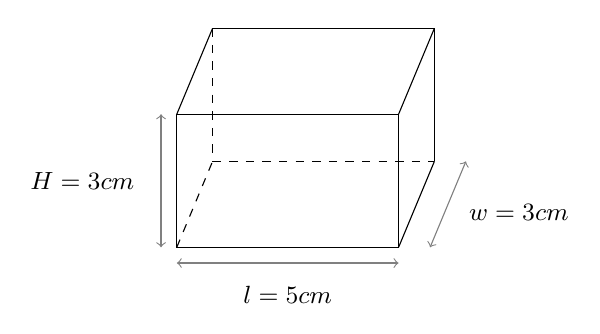
\begin{tikzpicture}[scale=1.0, baseline=(current bounding box.north)]
    \begin{scope}[rotate=0]

    % front face
    \coordinate (K) at (0,0);
    \coordinate (L) at (2.817,0);
    \coordinate (M) at (2.817,1.69);
    \coordinate (N) at (0,1.69);

    % back face skew shift
    \coordinate (Q) at ($(K)+(0.455, 1.092)$);
    \coordinate (R) at ($(L)+(0.455, 1.092)$);
    \coordinate (S) at ($(M)+(0.455, 1.092)$);
    \coordinate (T) at ($(N)+(0.455, 1.092)$);

    % draw prism edges
    \draw[] (K)--(L)--(M)--(N)--cycle;
    \draw[dashed] (K)--(Q);
    \draw[] (L)--(R);
    \draw[] (M)--(S);
    \draw[] (N)--(T);
    \draw[dashed] (Q)--(R);
    \draw[] (R)--(S);
    \draw[] (S)--(T);
    \draw[dashed] (T)--(Q);

    % label corners
    % \node[above left] at (K) {K};
    % \node[below right] at (L) {L};
    % \node[above right] at (M) {M};
    % \node[above left] at (N) {N};
    % \node[below left] at (Q) {Q};
    % \node[below right] at (R) {R};
    % \node[above right] at (S) {S};
    % \node[above left] at (T) {T};

    % dimension lines enabled
    \coordinate (P1offAB) at ($ (K)+(0,-0.2) $);
    \coordinate (P2offAB) at ($ (L)+(0,-0.2) $);
    \draw[<->,gray] (P1offAB)--(P2offAB);
    \node[black, fill=white, fill opacity=1.0, text opacity=1, inner sep=1pt]
        at ($ (P1offAB)!0.5!(P2offAB) + (0,-0.4) $) {\small $l=5 cm$};

    \coordinate (P1offAD) at ($ (K)+(-0.2,0) $);
    \coordinate (P2offAD) at ($ (N)+(-0.2,0) $);
    \draw[<->,gray] (P1offAD)--(P2offAD);
    \node[black, fill=white, fill opacity=1.0, text opacity=1, inner sep=1pt]
        at ($ (P1offAD)!0.5!(P2offAD) + (-1.0,0) $) {\small $H=3 cm$};

    \coordinate (P1offBF) at ($ (L)+(0.4,0) $);
    \coordinate (P2offBF) at ($ (R)+(0.4,0) $);
    \draw[<->,gray] (P1offBF)--(P2offBF);
    \node[black, fill=white, fill opacity=1.0, text opacity=1, inner sep=1pt]
        at ($ (P1offBF)!0.5!(P2offBF) + (0.9,-0.10) $) {\small $w=3 cm$};
    \end{scope}
\end{tikzpicture}
\end{minipage}
\hfill
\begin{minipage}{.5\textwidth}
  \begin{align*}
  \text{Volume} &= lwH \\
  \text{Volume} &= \dotuline{~~~~~} \,\text{cm} \times \dotuline{~~~~~} \,\text{cm} \times \dotuline{~~~~~} \,\text{cm} \\
  \text{Volume} &= \dotuline{~~~~~} \,\text{cm}^3
  \end{align*}
\end{minipage}

\end{document}

